\documentclass[letterpaper, 10pt, conference]{ieeeconf}

\IEEEoverridecommandlockouts                              % This command is only
                                                          % needed if you want to
                                                          % use the \thanks command
\overrideIEEEmargins
% See the \addtolength command later in the file to balance the column lengths
% on the last page of the document

\addtolength{\textfloatsep}{-4mm}	% reduce the space between figures and text
%\addtolength{\floatsep}{-3.6mm}		% reduce the space between figures

%=================================================================%
% Packages
\usepackage{amsmath,amssymb,amsfonts,bbm} % math
\usepackage{algorithm,algorithmicx,listings}  % algorithms
\usepackage[noend]{algpseudocode}			  % necessary for algorithmicx
\usepackage{url}					  % url citing
\usepackage{graphics,graphicx,subfigure,color}	%figures and color	

%\let\labelindent\relax				% allows using enumitem with IEEEconf
%\usepackage{enumitem}				% named bullets
%\usepackage{array,multirow,caption}			% table sutff
%\usepackage{tikz}
%\usetikzlibrary{arrows,petri,topaths,automata}
\usepackage{gensymb}		% \degree

% Bharath ADDONS:
\usepackage{setspace}
\usepackage{verbatim} %for multiline comment
\usepackage[mathscr]{euscript}
\usepackage[pdftex]{epsfig}

%\usepackage[usenames,dvips,pdftex]{color}
%\usepackage[pdftex]{color,graphicx}

%\usepackage{subfig}
%\usepackage{subfigure}
%\usepackage{sty/algorithm}
%\RequirePackage{setspace}
%\usepackage{captcont}

%\usepackage{multirow}

%\usepackage[square]{natbib}



%=================================================================%
% Commands
\def\liminf{\mathop{\lim\,\inf}\limits}	% EXAMPLE: \liminf_n A_n
\def\limsup{\mathop{\lim\,\sup}\limits}	%
\def\argmin{\mathop{\arg\,\min}\limits}	%
\def\argmax{\mathop{\arg\,\max}\limits}	%
\newcommand{\indicator}{\mathbbm{1}}
\newcommand{\txbx}[1]{\boxed{\text{#1}}}

\newtheorem{thm}{Theorem}
\newtheorem{proposition}{Proposition}
\newtheorem{definition}{Definition}
\newtheorem{assumption}{Assumption}
\newtheorem{remark}{Remark}
\newtheorem{problem}{Problem}



\begin{document}

%===================== TITLE =========================%
\title{\LARGE \bf A Policy gradient approach for interactive segmentation}

\author{Bharath Sankaran, Mrinal Kalakrishnan, Jeannette Bohg, Stefan Schaal% <-this % stops a space
\thanks{This work was supported by the }% <-this % stops a space
\thanks{B. Sankaran, M. Kalakrishnan and S.Schaal are with the Computational Learning and Motor Control Lab, University of Southern California, Los Angeles, CA 90089, {\tt\small bsankara@usc.edu, kalakris@usc.edu}}%
\thanks{J.Bohg and S.Schaal are with the Autonomous Motion Department, Max Planck Institute for Intelligent Systems, Tuebingen Germany, {\tt\small jbohg@mpi-is.de,sschaal@mpi-is.de}}%
}
\maketitle
%======================================================%

%\thispagestyle{empty}
%\pagestyle{empty}

\begin{abstract}
The paper is about a really cool idea on how to incorporate the action models to achieve perceptual tasks
\end{abstract}

%\section{Introduction}
\section{Introduction}
\label{sec:intro}
Personal robots need to have the ability to intelligently interact with their environments to be able to successfully operate in human environments. In this paper we focus on a specific class of intelligent interaction; namely the ability to pick the most optimal action given any perceptual input and adapt this action selection model online, to any variation in inputs. Most autonomous systems engaging in forceful interaction with the environment are tasked with this fundamental problem of action selection, i.e given the current perceptual input what is the most optimal action to select to achieve some given objective. When the objective of such tasks is strictly perceptual the task of action selection can be cast into either of one of the two classes of problems:\\
\begin{enumerate}
 \item Active Perception : Agent's actions do not change the physical state of the environment\\ 
 \item Interactive Perception : Agent's actions can change the physical state of the environment\\
\end{enumerate}

The problem of active perception for visual input has been one that has been long studied in the computer vision community since the early 80s. The multiple flavors of active perception such as sensor management, next best view, PTZ-control deal with the fundamental problem of how to control the sensor to achieve some perceptual objective. In previous work the problem of active perception for object detection was addressed by Sankaran and Atanasov (\cite{Javidi12_Journal}: TODO: Fix citiation to ICRA '13). In the current work we look at addressing the problem of interactive perception, specifically the problem of clutter segmentation.  

The problem of clutter segmentation is an interactive perception problem as every action the agent selects to declutter the environment changes the physical state of the environment. In this domain of clutter segmentation, we assume no prior knowledge of any objects in the environment. The action selection in our approach is restricted to a set of movement primitives that can be executed at any location in the environment. These movement primitives can include actions like grasping, pushing, pulling etc.

\begin{figure}[ht!]
	\centering
	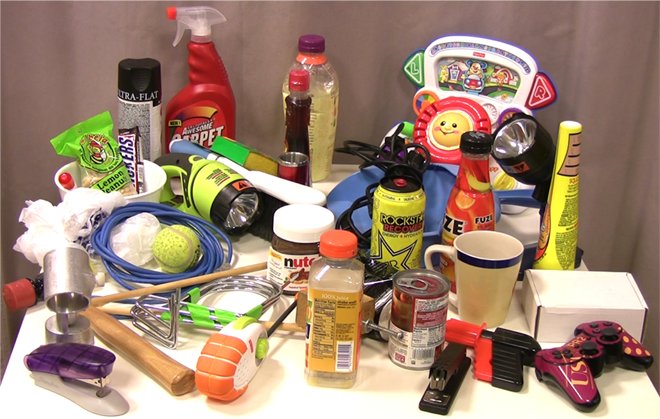
\includegraphics[width=\linewidth]{figs/clutter.png}
	\caption{Robot Operating in Clutter: TODO: Put in a better picture}
	\label{fig:intro}
\end{figure}
%[TODO: Insert picture of experimental setup from simulation]

% With the rapid progress of robotics research, the utility of autonomous robots is no longer restricted to controlled industrial environments. The focus has shifted to high-level interactive tasks in complex environments. The effective execution of such tasks requires the addition of semantic information to the traditional traversability representation of the environment. For example, a household robot needs to be able to detect an object of interest among those scattered on a dining table. For manipulation, it needs to estimate the object's pose accurately.
% 
% One of the central problems in computer vision, object detection and pose estimation, historically has been addressed with the assumption that the position of the sensing device is fixed \cite{Lowe04}, \cite{BelongieMP02}, \cite{FanMN89}. However, occlusions, variations in lighting, and imperfect object models in realistic environments decrease the accuracy of single-view object detectors. 
% 
% Active perception approaches circumvent these issues by utilizing appropriate sensing settings to gain more information about the scene. A large body of research in \textit{sensor management} \cite{Hero11_sensor_management} presents a structured approach to controlling the degrees of freedom in sensor systems and satisfying operational constraints while achieving the task objectives. However, most of the work either assumes  a simplified model for the detection process \cite{spaan08_POMDP, Jenkins10_PhD} or avoids the problem altogether and concentrates on estimating a target's state after its detection \cite{Hero03_sensor_management, sommerlade08_information, Mihaylova03_active_sensing}.
% 
% This paper is a step towards bridging the gap between the research in sensor management and the recent advances in 3D object detection enabled by the advent of low cost RGB-D cameras and open-source point cloud libraries \cite{Rusu_ICRA2011_PCL}. Rather than placing the burden of providing perfect results on a static detector, the sensor can move to increase the confidence in its detection. We consider the following problem. A mobile sensor has access to the models of several objects of interest. Its task is to determine which, if any, of the objects of interest are present on a cluttered table and to estimate their poses. The sensor has to balance the detection accuracy with the time spent observing the objects. The problem can be split into a static detection stage followed by a planning stage to determine a sequence of points of view, which minimize the mistakes made by the observer.
% 
% The rest of the paper is organized as follows. The next section provides an overview of related approaches to active object detection and summarizes our contribution. In section \ref{sec:problem} we draw up hypotheses about the class and orientation of an unknown object and formulate the active detection problem precisely. Section \ref{sec:obj_detect} describes our approach to static detection using a depth camera. In section \ref{sec:obs_model} we discuss the generation of an observation model, which is used in a Bayesian framework to assign a confidence measure on the hypotheses. Section \ref{sec:hyp_test} presents a formalism, which allows testing the hypotheses based on the sensor's observations and selecting a sequence of view-points to balance the sensing time with the decision accuracy. Implementation details are discussed in Section \ref{sec:impl_det}. Finally, in section \ref{sec:experiments} we present simulation results and discuss the validity of our approach.

%\newpage

%\begin{enumerate}
%	\item Why is the problem important? Give motivation and introduction!
%	\item Explain the scenario considered  and the approach to solving the problem
%	\item Talk about other approaches and differentiate the work from them
%	\item Explain the contributions and importance of the work
%\end{enumerate}

%As a result of the latest advances in robotics research, robots are beginning to move away from traditional tightly controlled industrial environments into more complex and dynamic environments. To effectively operate in these environments, the focus of robotic task specification has shifted towards more high-level interactive tasks. For the successful execution of these tasks, the robot requires additional semantic information to be incorporated into the traditional traversibility representations of the environment. For example, a household robot that needs clear a table has to be able to determine if there are any bottles among the objects present on the table. Upon the detection of such objects of interest the robot also needs to estimate the pose accurately enough to manipulate these objects.
%need to detect objects of interest and estimate their location and orientation accurately enough for grasping and manipulation tasks.


%One of the central problems in \textit{computer vision} is object detection and pose estimation. This problem when incorporated into high level task specification also requires the efficient estimation of semantic context with respect to the task. Historically, object detection and pose detection has been addressed with the assumption that the positions of the sensors are fixed ~\cite{Lowe04},~\cite{BelongieMP02} and ~\cite{FanMN89}
%Though there have been a wide variety of techniques developed to address the stationary sensor case, it still remains an open problem as it is consistently plagued by false positives and false negatives. Attempting to develop a perfect object detector for a single viewpoint is an unrealistic task for real world environments as occlusions, variations in lighting and imperfect object models limit the detection capabilities of most algorithms.

%Object recognition is one of the core problems in computer vision, and it is a very extensively investigated topic. Due to appearance variabilities caused for example by non-rigidity, background clutter, differences in viewpoint, orientation, scale or lighting conditions, it is a hard problem.

%Object occlusions, poor lighting or ambiguities of object models limit the detection capabilities of any approach that relies on a single point of view. 


%This paper is a step towards bridging the gap between the research in sensor management while utilizing state of the art techniques in 3D object detection which have gained traction since the advent of low cost RGB-D cameras and the availability of open source libaries for 3D object detection ~\cite{Rusu_ICRA2011_PCL}. Rather than relying entirely on the object detector for perfect estimation, the mobile sensor can execute appropriate actions to improve its detection.


%\section{Related Work}
\section{Related Work}
\label{sec:rel_work}
{\bf The related work needs to be written from scratch. The stuff written below is from another previous paper and is being used as a place holder.} The approaches in sensor management \cite{Hero11_sensor_management, Huber09_PhD} can be classified according to sensor type into \textit{mobile} (sensors have dynamic states) and \textit{stationary} (sensors have fixed states). Also, the targets of interest might be mobile or stationary. The process of choosing sensor configurations may quantify the utility of the next configuration only (\textit{myopic}) or may optimize over a sequence of future sensor configurations (\textit{non-myopic}). Finally, the objective may be to identify a target and estimate its state or simply improve the state estimate of a detected target.

The earliest work in active perception can be attributed to Bajscy \cite{bajscy_88, Krotkov_93}. It was focused on 3D position estimation through control of the sensor's intrinsic parameters. Pito's 1999 paper \cite{pito99_nbv} addresses the next best view problem as one that maximizes information gain by increasing spatial resolution. The movement of the sensor is constrained to a circle centered around the object of interest.

The work that is closest to ours \cite{Scharinger10_SceneModeling6D} uses a mobile sensor to classify stationary objects on a table and estimate their poses. Static detection is performed using SIFT matching. An object's pose distribution is represented with a Gaussian mixture. The authors use a myopic strategy to reduce the differential entropy in the pose and class distributions. This work differs from ours in that the sensor has models of all the objects so the detection is never against background. Moreover, by formulating hypotheses about an object's identity and by choosing a small discrete space for the possible sensor poses, we are able to plan non-myopically.

Velez and coworkers \cite{velez11_ijcai, velez11_icaps} consider the problem of detecting doorways, while a mobile sensor is traveling towards a fixed goal point. The unknown state of a candidate detection is binary: "present" or "not present". Stereo disparity and plane fitting are used for pose estimation. An entropy field is computed empirically for all view-points in the workspace and is used to myopically select locations with high expected information gain. The authors assume that the static detector provides sufficiently accurate pose estimates and do not optimize them during the planning.

In our work we use a depth sensor, which validates the assumption that the position estimate of a stationary object is accurate and does not need to included in the optimization objective. However, the orientation estimates can be improved through active planning. Inspired by the work on hypothesis testing \cite{Javidi12_arxiv}, we introduce a rough discretization of the space of orientations so that the hidden object state takes on several values, one for "object not present" and the rest for "object present" with a specific orientation. As a post-processing step, the rough orientation estimate is used to seed a robust alignment procedure, which provides an accurate pose estimate. In our previous work we considered a dual hypothesis problem aimed at model completion \cite{BharathThesis}. 

Karasev et al. \cite{karasev12_visual_learning} plan the path of a mobile sensor for visual search of an object in an otherwise known and static scene. The problem statement is different from ours but the optimization is surprisingly similar. The authors hypothesize about the pose of the object and minimize the probability of an incorrect decision. Since different object locations need to be considered, the optimization is intractable. Instead, a mathematical model of the sensing process is used to maximize the conditional entropy of the next measurement. 
 
A lot of the work in sensor management assumes a fixed sensor position, which simplifies the problem considerably because the trade-off between minimizing movement energy and maximizing view-point informativeness is avoided \cite{sommerlade08_information, Kragic06_ActiveObjRecognition}. Often, the action selection process is myopic. In contrast, we consider a mobile sensor, include the detection process in the optimization, and use non-myopic planning. Golovin and Krause \cite{golovin11_adaptive} showed that myopic planning for an adaptively submodular objective function is merely by a constant factor worse than the optimal strategy. Unfortunately, the objective in our formulation is not adaptively submodular and even with a fixed sensor state, a myopic strategy can perform arbitrarily worse than the optimal policy \cite{Javidi12_arxiv}.

The contributions of this paper are two-fold. Firstly, we introduce the idea of implicit pose estimation in 3D object detection by utilizing a vocabulary tree-based partial view matching. In addition to detecting the object's class this approach allows us to retrieve a course pose estimate. Moreover, relying on partial views helps in scenarios in which the object of interest is either partially occluded or in contact with another object. Secondly, we introduce a formal hypothesis testing framework to improve upon the static detection results by moving the sensor to more informative view-points. Our non-myopic planning approach weights the benefit of gaining more certainty about the correct hypothesis against the physical cost of moving the sensor. 




%we integrate static object detection using a real depth sensor with a non-myopic planning approach which performs hypothesis testing. Our formal hypothesis testing framework weights the benefits of gaining more certainty about the existence of an object against the physical cost of moving to more informative viewpoints and explicitly minimizes the number of false positive and false negative mistakes.



%A lot of the work in the sensor management field assumes a fixed sensor position, which simplifies the problem considerably because the trade-off between minimizing the movement energy and maximizing the view-point informativeness is avoided. For example, the authors of \cite{sommerlade08_information} control the pan, tilt, and zoom of a camera in order to track mobile targets, whose detection is assumed to be solved. Kalman filters are used to estimate the target states and the camera parameters are set to minimize the conditional entropy of the scene model. Similarly, Ekvall et al. \cite{Kragic06_ActiveObjRecognition} control a pan-zoom-tilt camera with a fixed position but include the detection process in their decision-making. The action selection process is myopic in both papers, while in our work we consider a mobile sensor, include the detection process in the optimization, and use a non-myopic planning process.






%we discuss approaches for generating an observation model specific to the task of object detection in a Bayes framework. Finally, 


%1) Using a point cloud data for static object detection and estimation
%2) Discussion several approaches to generate an observation model specific to the task of object detection
%3) Connecting static object detection and estimation using RGB-D camera to a formal hypothesis testing framework. 


%The following papers are relevant: \cite{Rhunke11_SparseSurfaceAlignment}, \cite{Roy12_EstPlanMap}, \cite{Shi11_MultiHypothesis}, \cite{Rusu10_ViewpointFeatureHistogram}, \cite{Fox11_JointObjPoseRecognition}, \cite{Fox11_ObjectRecognition}.

%Some of the exemplary papers in sensor management include \cite{Hero03_sensor_management}, in which the goal of the system is to learn the number and states of a group of moving targets occupying a surveillance region. A good measure of the quality of a sensing action is the reduction in entropy of the posterior distribution that is induced by the measurement.

%(POMDP Myopic)
%Approaches in active vision go to the other extreme, where the mobility and cost functions are modelled using a general POMDP formulation \cite{spaan08_POMDP}, \cite{Mihaylova03_active_sensing}, \cite{Scharinger10_SceneModeling6D}, \cite{Hero03_sensor_management}. Since the strucutre of the problem is not utilized the optimization problem is intractable and the authors are forced to resort to myopic planning.

%(Soatto) 
%The authors of \cite{valente12_info_gathering} are interested in designing a path through space, at the end of which the viewer will have seen all obstacles in an unknown environment. This problem is quite different from object detection and estimation but from a planning perspective it contains interesting ideas. The authors define an accumulated visibility level set function, which encodes the knowledge that the viewer has of the environment when moving along a given path and otian it as a solition to an Eikonal PDE.

%(Sukhatme) 
%The authors of \cite{Potthast11_NextBestView} consider an information gain-based variant of the next best view problem. A mobile sensor is tasked to sequentially take scans of an initially unknown environment with the objective of rapidly decreasing the amount of unknown space. A belief model for the visibility of the occluded space is used to predict the potential gains of different actions and a myopic planning scheme is used to select the best one.











%Our hypothesis testing framework selects sequences of actions, which explicitly minimze the number of false positive and false negative mistakes made by the detector and 

%Second, we introduce a formal hypothesis testing framework to select a sequence of actions, which explicitly minimze the number of false positive and false negative mistakes. Our non-myopic planning scheme weights the benefits of gaining more certainty about the existence of an object against the physical cost of moving to more informative viewpoints.
%to select a sequence of actions, which improves the belief of a detection obtained from a static object detector. 

%Our formal planning framework is based on the theoretical research in active multi-hypothesis testing presented in \cite{Javidi10_MaryHypothesisTesting, Javidi10_HypothesisTesting, Javidi11_HypothesisTesting, Javidi12_Journal}, which weights the benefits of gaining more certainty about the existence of an object against the physical cost of moving to different viewpoints.

%The goal of this paper is to integrate static object detection using a real RGB-D sensor with an active planning framework, which selectes sequences of opimal sensor poses and explicitly minimizes the number of false positive and false negative mistakes. This requires a number of complex modifications over the classical \textit{sensor management} problem:
% - complex observation model suitable for a detection tasks
% - introduce mobility and minimize cost of movement in a nonmyopic planning framework



















%DONE:
%\cite{Javidi10_HypothesisTesting}, \cite{sommerlade08_information}, \cite{spaan08_POMDP}, \cite{Hero03_sensor_management}, \cite{Mihaylova03_active_sensing}, \cite{valente12_info_gathering}, \cite{velez11_ijcai}, \cite{Herbst11_icra}, \cite{Jenkins10_PhD}, \cite{Lehment11_HumanPoseTracking}, \cite{Fallon12_SceneSimulation}, \cite{Potthast11_NextBestView}, \cite{Kragic06_ActiveObjRecognition}, \cite{Cipolla04_TemplateLikelihood}, \cite{Scharinger10_SceneModeling6D}.


%From a motion planning perspective the closest work to ours is [Velez]. Velez and coworkers descirbe an online, any-time planning framework using a mobile sensor for object detection. The unknown state of the object is a binary random variable, which takes on the values "present" and "not present". The authors formulate a binary hypothesis testing problem, which weights the benefit of increasing the confidece in the state of the hidden variable against the cost of taking a detour to reach an informative view.

%However, the problem formulation is abandoned and instead the conditional entropy between the state of the object and the confidence of the object detector is computed empirically for all viewpoints in the robot's workspace. This field is used to bias the planning towards locations with high expected information gain. It is not clear what is the relationship between minimizing this entropy field and the cost function in the original formulation, which minimizes the number of false positive and false negative mistakes explicitly.

%The authors assume that the detector can estimate the postion and orientation of the detected object accurately enough. Their problem formulation does not optimize over the quality of the estimation. 

%In our work we use a depth sensor, which validates the assumption that the position of the object can be estimated well enough without explicit inclusion in the optimization problem. However, ignoring the orientation of the object in the opitmization is not desirable because the results of static orientation estimation can be significantly improved using active planning. Reasoning over the continuous space of orientations is intractable. Instead, we introduce a very rough discretization of the space of orientations and note that it is sufficient because a post-processing step based on template matching can be used to obtain a very accurate orientation estimate. Thus, in our formulation the hidden object state takes on several integer values, one for "object not present" and the rest for "object present" with a specific orientation. 
%This leads to an active M-ary hypothesis testing problem with a mobile sensor. To our knowledge this formulation has not been addressed in literature and the closest work is Javidi in which the state of the sensor is fixed.

%Velez and coworkers \cite{velez11_ijcai, velez11_icaps} consider the problem of enriching metric maps with semantic information. In particular, a mobile sensor attempts to detect doorways along its way to a fixed goal point. The agent weights the benefit of increasing its confidence about a detection against the cost of taking a detour to a more suitable vantage point.

%The authors utilize a static object detector due to \cite{Felzenszwalb08_detector} and use stereo disparity and plane fitting to estimate the position and orientation of detected doorways. They utilize a non-myopic action selection strategy, which minimizes the entropy between a detection hypothesis and the confidence of the object detector. Our planning stage is similar... (DESCRIBE HOW IT IS DIFFERENT)












%Conversely, a large body of research has focused on 

%Even state-of-the-art approaches to the static object detection are affected adversely by 

%object detectors  Regardless of how good object detectors 


%A straightfor-
%ward approach to adding semantic information is to accept
%the results of a standard object detector framework prima fa-
%cie, irrespective of sensor noise.

%As robotic research progresses, autonomous robots are used to perform high-level tasks in complex and dynamic environments. Sophisticated interactions between an agent and its workspace 


%These tasks are very important for precise grasping an manipulation 

%The progress of robotics research is indicated by 
%The success of the 
%One of the central problems of computer vision is the detection of semantically important objects and the estimation of their pose and shape information.


%objects and activities.

%Inaccurate sensing devices, bad classifiers, object occlusions, poor lighting or ambiguities of object models limit the detection capabilities. Active perception approaches aim at deliberately utilizing appropriate sensing settings to gain more information about the scene.


%Detecting objects, estimating their pose and recovering 3D shape information are critical problems in many vision and robotics applications


%* Useful for grasping and object manipulation. This information will help the robotic arm grasp the object at the right location and successfully interact with it.
%* Useful for incorporating semantic information into SLAM / metric maps

%* Active object detection is natural to humans and animals, while in the robotics and computer vision communities more emphasis has been placed on static object detection. However, attempting to develop a perfect object detector for a fixed viewpoint is a hopeless task for realistic environments, where occlusions, lighting, and changes affect the view.

%* The object detection problem is hard

%* One of the central problems of Computer Vision is the detection and estimation of objects and activities.

%In this paper we address the problem of detecting an object and estimating its position and orientation. Moreover, our approach is active. The sensor can use a set of motion primitives to move in the environment.

%Including mobility in object detection is crucial for the advancement. For example, authers of lbalbla showed that using a realtively weak detector in an active framework can lead to a significant performance improvement. 

%We address the problem of 3D object detection from point cloud data. The use of point cloud data has gained immense popularity in the vision research communities with the advent of the RGB-D cameras and the open source Point Cloud Library.
% 
%% 1. Importance and motivation for object recognition
%The wide availability of RGB-D cameras


%\section{Problem Formulation}
\section{Problem Formulation}
\label{sec:problem}
Consider a set of rigid objects piled-up on any surface denoted $T_1,...,T_n \in \mathcal{T}$, where n is the number of objects. This set of rigid objects can be represented by a graph $\mathcal{G}$ where each vertex $g_i \in \mathcal{G}$ corresponds to a node with unique appearance. Here appearance can be defined by a number different attributes combined into a feature vector.

Every object in our set $\mathcal{T}$ can be represented by a rigid clique in this graph $\mathcal{G}$ comprising of one or more interconnected nodes $g_i$. Edges between rigid cliques are dynamic edges which are removed when two rigid objects are separated. Hence each rigid object corresponds to a set of nodes $\{g_{i1},..g_{in}\}$ in a clique $\mathcal{C}_i$. A collection of such cliques with 

with edges between them represents our scene graph denoted by $\mathcal{G}$. We cast the clutter segmentation problem as a graph separation problem where our objective is to pick a set of minimal actions to remove the dynamic edges from the graph and separate the graph into a set of minimal cliques each of which represent a rigid body.

In the initialization phase the dynamic edges between cliques represent the rigid objects that are either touching each other or entagled with each other in a pile of objects.

Given an initial scene graph $\mathcal{G}$ our objective is to pick the most optimal sequence of actions from a discrete set of actions $\{a_1,....a_m\} \in \mathcal{A}$ which optimizes the objective of graph separation and reduces the number of actions required to be executed. As the problem of trying to identify the set of actions that optimizes

the graph separation objective for the set of all possible graphs is intractable (given all possible set of graphs that one might encouter in natural scenes). To circumvent this problem we try to learn a mapping from actions $\mathcal{A}$ to features $\mathcal{F}$. These features $\mathcal{F}$ represent the current state of the environment. Instead of mapping actions to graphs we constraint the problem by trying

to learn a mapping between actions $\mathcal{A}$ and features $\mathcal{F}$. The quality of the features can be evaluated by the reward observed after executing each action. This learning problem can be cast as a supervised learning problem to classify the features based on action labels. Our learning approach discussed in detail Section \ref{sec:hyp_test}. Since we need to label features, we use Learning from 

Demonstration (LfD) to execute actions and label them with user specified rewards. We use a Max Entropy learner as the dimensionalty of the feature vector we use is much larger compared to the number of samples we collect.

As the dimensionalty of the feature space is incredibly high, we may still not be able to capture the entire variance in the feature space. To account for this variation, we let the learner adapt online to the features. Hence we utilize an online policy gradient styled approach where we optimized parametrized actions with respect to an expected reward by gradient descent. The details of the approach are dicussed in Section \ref{sec:hyp_test}.



% Let the table surface be represented by a bounded set $\mathcal{T} \subset \mathbb{R}^2$. Let $B_0$ be the possibly infinite set of all object classes that may appear on the table. We assume that each object class has a single model associated with it and use the words model and class interchangeably. Instances are drawn from $B_0$ at random and are placed uniformly on the table surface. For simplicity we assume that the objects have a random yaw and no pitch or roll so that their poses are in $SE(2)$. The extension of our framework to the $SE(3)$ case is immediate.
% 
% Consider a mobile depth sensor, whose position and orientation at time $t$ are $x_t = (x_t^p,x_t^r) \in SE(3)$. Let $\Omega$ represent the state of the \textit{static} environment, which includes factors such as scene geometry, lighting, occlusion, etc. At time $t$, the depth sensor can obtain a point cloud $\mathcal{Q}_t \subset \mathbb{R}^3$ from the scene which is visible from $x_t$ according to $\mathcal{Q}_t = \phi(x_t,\Omega)$. The first task of the sensor is to split $\mathcal{Q}_t$ into separate surfaces (\textit{segmentation}) and associate them with either new or previously observed objects (\textit{data association}). These procedures are not the focus of our paper but we mention briefly how we perform them in Subsection \ref{subsec:seg_data_ass}. We assume that they estimate the object positions accurately. 
% 
% The sensor has access to a database of size $L_1 < \infty$ of object models $B_1 \subset B_0$ and a subset $B_2 = \{C_1,\ldots,C_{L_2}\} \subseteq B_1$ of them are designated as objects of interest. The task of the sensor is to detect all objects from $B_2$, which are present on the table and to estimate their pose as \textit{quickly} as possible. Note that the detection is both against known objects from $B_1$ and unknown background from $B_0 \setminus B_1$.
% 
% We are interested in choosing a sequence of view-points for the mobile sensor, which has an optimal trade-off between energy used to move and number of incorrect classifications. Doing this with respect to all objects simultaneously results in a complex joint optimization problem. Instead, we treat the objects independently and process them sequentially, which simplifies the task to choosing a sequence of sensor poses with respect to a single object.
% 
% Further, we restrict the motion of the sensor to a sphere $S^2(\rho)$ of radius $\rho$, centered at the location of the object. The sensor's orientation is fixed so that it points at the centroid of the object. We denote this space of sensor poses by $V(\rho)$ and refer to it as a \textit{viewsphere}. A sensor pose $x \in V(\rho)$ is called a \textit{viewpoint}. As a result, we only need to plan for a sequence of viewpoints. At a high-level planning stage we assume that we can work with a fully actuated model of the sensor dynamics so that for any two poses $x^1, x^2 \in V(\rho)$, there exists a control $u^{1,2} \in U$, which takes the sensor from $x^1$ to $x^2$. At time $t$ the sensor can either move and make one more observation or decide on the class and orientation of the unknown object and retire.
% 
% As mentioned in Section \ref{sec:rel_work}, the space of object orientations is discretized sparsely as $\Theta = \{r_1,\ldots, r_N\} \subset SO(2)$. Thus, the hidden variables in the single object optimization are the object class $Y \in B_2$ and the object orientation $R \in \Theta$. The sensor needs to decide between $M = L_2 N + 1$ hypotheses:
% \begin{align*}
% H_0:&\text{ the object does not belong to $B_2$,}\\
% H_i:&\text{ the object is of class $\textit{cl}(H_i) := C_{mod(i,L_2)} \in B_2$}\\
% &\text{ with orientation $\textit{or}(H_i):= r_{(i-\textit{cl}(H_i))/L_2} \in \Theta$ for}\\
% &\; i = 1,\ldots,L_2 N
% \end{align*}
% In order to measure how well the task has been carried out we introduce the following costs:
% \begin{align*}
% \Lambda_{ij}&= \text{ cost for deciding on $H_i$, when $H_j$ is correct}\\
% &= \begin{cases}
%   		d(\textit{or}(H_i), \textit{or}(H_j)) & \textit{cl}(H_i) = \textit{cl}(H_j) \in B_2\\
%   		\Lambda_{fn} & \textit{cl}(H_i) \neq \textit{cl}(H_j) \in B_2\\
%   		\Lambda_{fp} & \textit{cl}(H_i) \in B_2, \textit{cl}(H_j) \in B_1 \setminus B_2\\
%   		0 & \text{if } i = j
%    \end{cases}\\
% c(x&^1,x^2) = d_{SE(3)}(x^1, x^2) + c_0 = \text{ cost of moving from $x^1$}\\
% & \qquad \text{to $x^2$ on the sphere and taking another observation}
% \end{align*}
% where $d_{SE(3)}(\cdot,\cdot)$ is a metric on $SE(3)$, $c_0 > 0$ is a fixed measurement cost, $\Lambda_{fp}$ and $\Lambda_{fn}$ are costs for making false positive and false negative mistakes respectively, and $d(\cdot,\cdot)$ is a cost for an incorrect orientation estimate, when the class is correct.
% 
% \begin{problem}[Active Object Detection]
% \label{prob:active_obj_detect}
% Given an object with random class $Y \in B_0$ and orientation $R \in SO(2)$ on the table $\mathcal{T} \ltimes SO(2)$, let $j^*(Y,R)$ denote the index of the hypothesis with the same class and closest orientation. The objective of the mobile sensor is to find a stopping time $\tau$, a sequence of viewpoints $x_0, \ldots, x_{\tau-1}$, and a decision rule $\delta(\mathcal{Q}_{1:\tau}) \in \{0,\ldots,M-1\}$ which minimize the cost:
% 
% \begin{align}
% \label{eq:sequential_optimization}
% \mathbb{E}_{\mathcal{Q}_{1:\tau},Y,R} \biggl\{ \sum_{t=0}^{\tau-1} c(x_t,x_{t-1}) + \Lambda_{\delta(\mathcal{Q}_{1:\tau}), j^*(Y,R)} \biggr\}.
% \end{align}
% \end{problem}
% 
% \begin{remark}
% The first term in (\ref{eq:sequential_optimization}) captures the energy spent moving, while the second term is a weighted probability of making a mistake. To see this suppose that all decision costs are equal, i.e. $D := d(\textit{or}(H_i), \textit{or}(H_j)) =\Lambda_{fn} = \Lambda_{fp}, \forall i,j$. Then:
% \begin{align*}
% \mathbb{E}_{\overset{\mathcal{Q}_{1:\tau},}{Y,R}}\biggl\{ \Lambda_{\delta(\mathcal{Q}_{1:\tau}), j^*(Y,R)} \biggr\} & = \mathbb{E}_{\overset{\mathcal{Q}_{1:\tau},}{Y,R}}\biggl\{ D \indicator_{\delta(\mathcal{Q}_{1:\tau}) \neq j^*(Y,R)}\biggr\}\\
% &= D \mathbb{P}( \delta \neq j^*),
% \end{align*}
% which is the probability that decision $\delta(\mathcal{Q}_{1:\tau})$ is incorrect. 
% \end{remark}
% 
% Our approach to solving the active object detection problem consists of two stages. First, we use a vocabulary tree to perform static detection in 3D. Since the detection scores are affected by sensor noise and occlusions we don't use them directly. Instead, we use a probabilistic framework to maintain the hypotheses about the detection outcome. In the second stage, we use non-myopic planing to select better viewpoints for the static detector and to update the probabilities of the hypotheses.





%\subsection{Object Detection}
%Our approach to object recognition involves extracting a set of templates $D = \{\mathcal{P}_1,\ldots,\mathcal{P}_G$ from the object model $\mathcal{M} \in B$. A template is extracted for each possible yaw $\theta \in R$ of the object of interest $\mathcal{M}$, by defining a set of viewpoints $V = \{v_1,\ldots,v_G\} \in S^2(\rho) \ltimes SO(3)$, which lie on a sphere of radius $\rho$ centered at the object. %where $\ltimes$ denotes a semidirect product


%Suppose that there is a finite number of three dimensional object classes $B = \{C_1,\ldots,C_L\}$ in the world. Object instances are drawn at random from $B$ and are placed uniformly on the table $\mathcal{T}$ with random yaw and no pitch or roll. We make the simplifying assumption that the object poses are in $SE(2)$ but the theoretical extension of our framework to the $SE(3)$ case is immediate given access to the model $\mathcal{M} \in B$ of one object of interest



%\section{Static Object Detection}
%\section{Observation Model}
\label{sec:obs_model}
% We would like to use a Bayesian framework to maintain probabilities for the object hypotheses. This requires statistics about the operation of the sensor for different object classes, orientations, and viewpoints. Instead of using the segmented pointcloud $\mathcal{Q}_t$ as the observation of the sensor, we take the output of the vocabulary tree. As a result, we deal with the space of possible vocabulary tree outputs rather than the space of all possible pointclouds. Moreover, this includes the operation of the vision algorithm in the sensor statistics. 
% 
% Given a query pointcloud $\mathcal{Q}_t$ suppose that the vocabulary tree returns template $\mathcal{P}_{g,l}$ as the top match. Assume that the models in the training database are indexed so that those from $B_2$ have a lower $l$ index than those from $B_1 \setminus B_2$. We take the linear index of the closest match $\mathcal{P}_{g,l}$ as the observation if the match is an object of interest. Otherwise, we record only the model index $l$, ignoring the viewpoint $g$:
% \[
% Z_t = \begin{cases}
% (l-1)G+g, & \text{if } l \leq L_2\\
% L_2G+(l-L_2), & \text{if } l > L_2, \forall g \in \{1,\ldots,G\}.
% \end{cases}
% \]
% This makes the observation space one dimensional. Given a sensor pose $x \in V(\rho)$ and an object hypothesis $H_i$, we need to approximate the data likelihood of $Z_t$:
% \[
% h_i^x(z) := \mathbb{P}(Z_t = z \mid x, H_i)
% \]
% The function $h$ is called the \textit{observation model} of the static detector. It can be obtained off-line since it only depends on the characteristics of the sensor and the vision algorithm. Ideally, the sensing and detection processes should be abstracted to obtain a closed-form representation of $h$ but this is a daunting task for a depth sensor and a vocabulary tree. Instead, we learn a histogram approximating $h$ using the training dataset $B_1$.
% 
% The viewsphere is discretized into a set of viewpoints $\mathcal{X}(\rho) \subset V(\rho)$, which will be used in the planning phase. It need \textit{not} be the same as the set $V_G(\rho)$ used to train the vocabulary tree. We generated $50$ random environments from the models in $B_1$ for each of the $7$ hypotheses and used a simulated depth sensor to obtain scores from the vocabulary tree for a set $\mathcal{X}(\rho)$ of $42$ viewpoints.


%\section{Obeservation Model}
\section{Observation Model}
\label{sec:obs_model}
% We would like to use a Bayesian framework to maintain probabilities for the object hypotheses. This requires statistics about the operation of the sensor for different object classes, orientations, and viewpoints. Instead of using the segmented pointcloud $\mathcal{Q}_t$ as the observation of the sensor, we take the output of the vocabulary tree. As a result, we deal with the space of possible vocabulary tree outputs rather than the space of all possible pointclouds. Moreover, this includes the operation of the vision algorithm in the sensor statistics. 
% 
% Given a query pointcloud $\mathcal{Q}_t$ suppose that the vocabulary tree returns template $\mathcal{P}_{g,l}$ as the top match. Assume that the models in the training database are indexed so that those from $B_2$ have a lower $l$ index than those from $B_1 \setminus B_2$. We take the linear index of the closest match $\mathcal{P}_{g,l}$ as the observation if the match is an object of interest. Otherwise, we record only the model index $l$, ignoring the viewpoint $g$:
% \[
% Z_t = \begin{cases}
% (l-1)G+g, & \text{if } l \leq L_2\\
% L_2G+(l-L_2), & \text{if } l > L_2, \forall g \in \{1,\ldots,G\}.
% \end{cases}
% \]
% This makes the observation space one dimensional. Given a sensor pose $x \in V(\rho)$ and an object hypothesis $H_i$, we need to approximate the data likelihood of $Z_t$:
% \[
% h_i^x(z) := \mathbb{P}(Z_t = z \mid x, H_i)
% \]
% The function $h$ is called the \textit{observation model} of the static detector. It can be obtained off-line since it only depends on the characteristics of the sensor and the vision algorithm. Ideally, the sensing and detection processes should be abstracted to obtain a closed-form representation of $h$ but this is a daunting task for a depth sensor and a vocabulary tree. Instead, we learn a histogram approximating $h$ using the training dataset $B_1$.
% 
% The viewsphere is discretized into a set of viewpoints $\mathcal{X}(\rho) \subset V(\rho)$, which will be used in the planning phase. It need \textit{not} be the same as the set $V_G(\rho)$ used to train the vocabulary tree. We generated $50$ random environments from the models in $B_1$ for each of the $7$ hypotheses and used a simulated depth sensor to obtain scores from the vocabulary tree for a set $\mathcal{X}(\rho)$ of $42$ viewpoints.


%\section{Active Hypothesis Testing}
\section{Online Adaptation}
\label{sec:hyp_test}
The online phase of the algorithm we create a scene graph $\mathcal{G} = \{V,E\}$, this graph at a selected vertex and update the action parametrization by updating the feature weights by gradient descent in feature space. The online phase of the algorithm has three stages; a supervised classification phase, a data association phase and an online gradient update phase. The three phases are discussed in detail in the sections below.
\subsection{Supervised Classification}
When a scene is presented to the agent (robot) in the form of an rgb image and corresponding point cloud is used to construct a scene graph $\mathcal{G}$. We first pre-process the point cloud to look for euclidean clusters supported by some dominant plane in the image. Once these clusters have been detected we project them back on to the image to get the corresponding image patches.

To construct the scene graph we oversegment these image patches in to superpixels using the graph based segmentation approach described in (\cite{Javidi12_Journal} TODO: Fix Citation). We then construct the scene graph by analyzing the nearest neighbours of each superpixel segment. Every vertex $V_i$ of the graph $\mathcal{G}$ would be correspond to a superpixel and the edges $E_j$ would be be drawn between superpixels touching each other. From such a respresentation the notion of rigid and dynamic edges are readily apparent as rigid edges are those edges that connect superpixels on the same object and dynamic edges are those edges that connect superpixels between two objects that are touching or in close proximity to each other. This is illustrated in the figure below Fig \ref{fig:scene_graph}.

\begin{figure}[ht!]
	\centering
	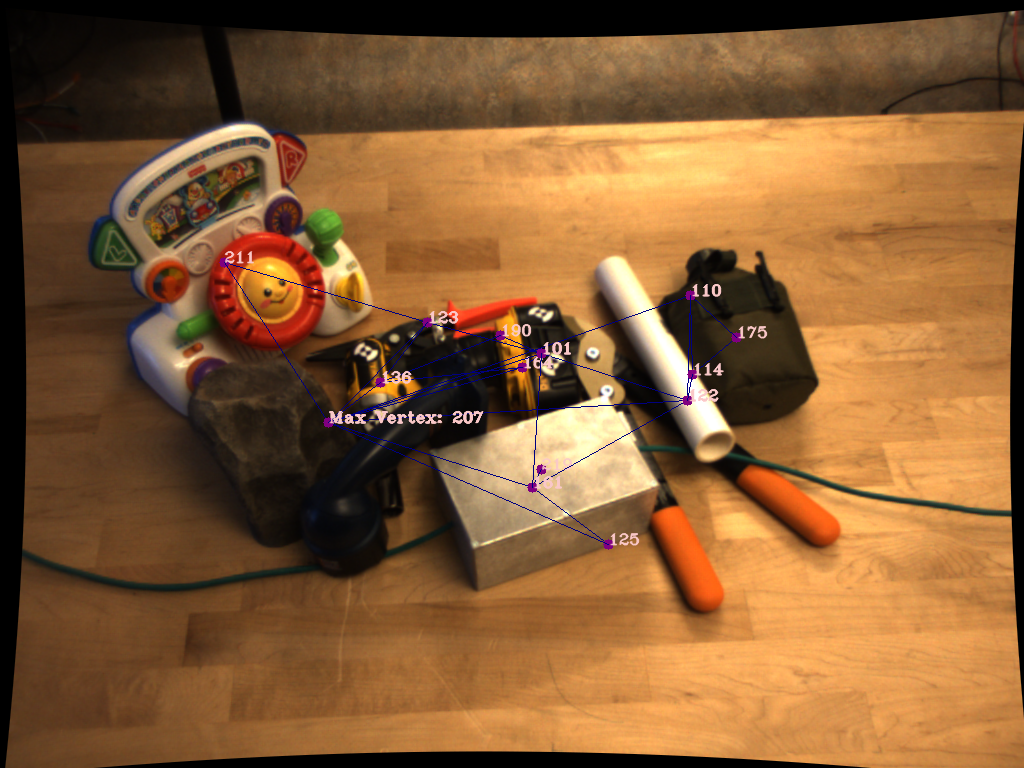
\includegraphics[width=\linewidth]{figs/full_graph.png}
	\caption{Illustrates the scene graph construction from a set of objects on a table}
	\label{fig:scene_graph}
\end{figure}

Once we generate the scene graph $\mathcal{G}$, we compute the set of features described in Section \ref{sec:lfd} for the vertex of maximum degree $V_{max}$ in the graph. The intuition for only attempting to manipulate the Vertex of maximum degree is that it is connected the most number of other vertices hence manipulating this vertex can impact the graph adjacency matrix more severly than any other node.

Once we compute the features for the max degree vertex $V_{max}$ we use the weights computed using the max entropy learner in the offline learning phase discussed in Section \ref{sec:lfd}. Using these weights we select the best action to execute by sampling the best action from a gibbs distribution as shown below.

\[
a_t = \max(\frac{\exp^{w^Tf(x)}}{ \sum_b\exp^{w^Tf(x)}})\\
\]

Once we generate the action to be executed we execute the action $a_t$ and observe the corresponding reward $R_t$. Here $t$ is the current time step and $f(x)$ is the feature function.

\subsection{Data Association}
Once the action is executed we track the vertices of the scene graph $\mathcal{G}_t$ using optical flow. The positions of the vertices of the graph are updated using the Gunnar Farnebaack Optical Flow algorithm (\cite{Javidi12_Journal} TODO: Cite Gunnars' ICPR 2000 paper) to obtain the predicted scene graph update $\tilde{\mathcal{G}}_{t+1}$. Once the vertices in the graph are updated to get the predicted graph $\tilde{\mathcal{G}}_{t+1}$, the predicted graph is matched with the observed scene graph $\hat{\mathcal{G}}_{t+1}$ to get the actual scene graph $\mathcal{G}_{t+1}$. The graph matching is accomplished by measuring the Bhattacharya distance given by

\[
D_B(p,q) = -\log{\sum_{x\in\mathcal{X}}\sqrt{p(x)q(x)}}\\
\]

between the appearance histograms of the vertices of each graph. Using this distance metric we are able to establish an accurate correspondence between $\tilde{\mathcal{G}}_{t+1}$ and $\hat{\mathcal{G}}_{t+1}$, to get $\mathcal{G}_{t+1}$. This correspondence matching is show below in Figure \ref{fig:correspondence}.

\begin{figure}[ht!]
	\centering
	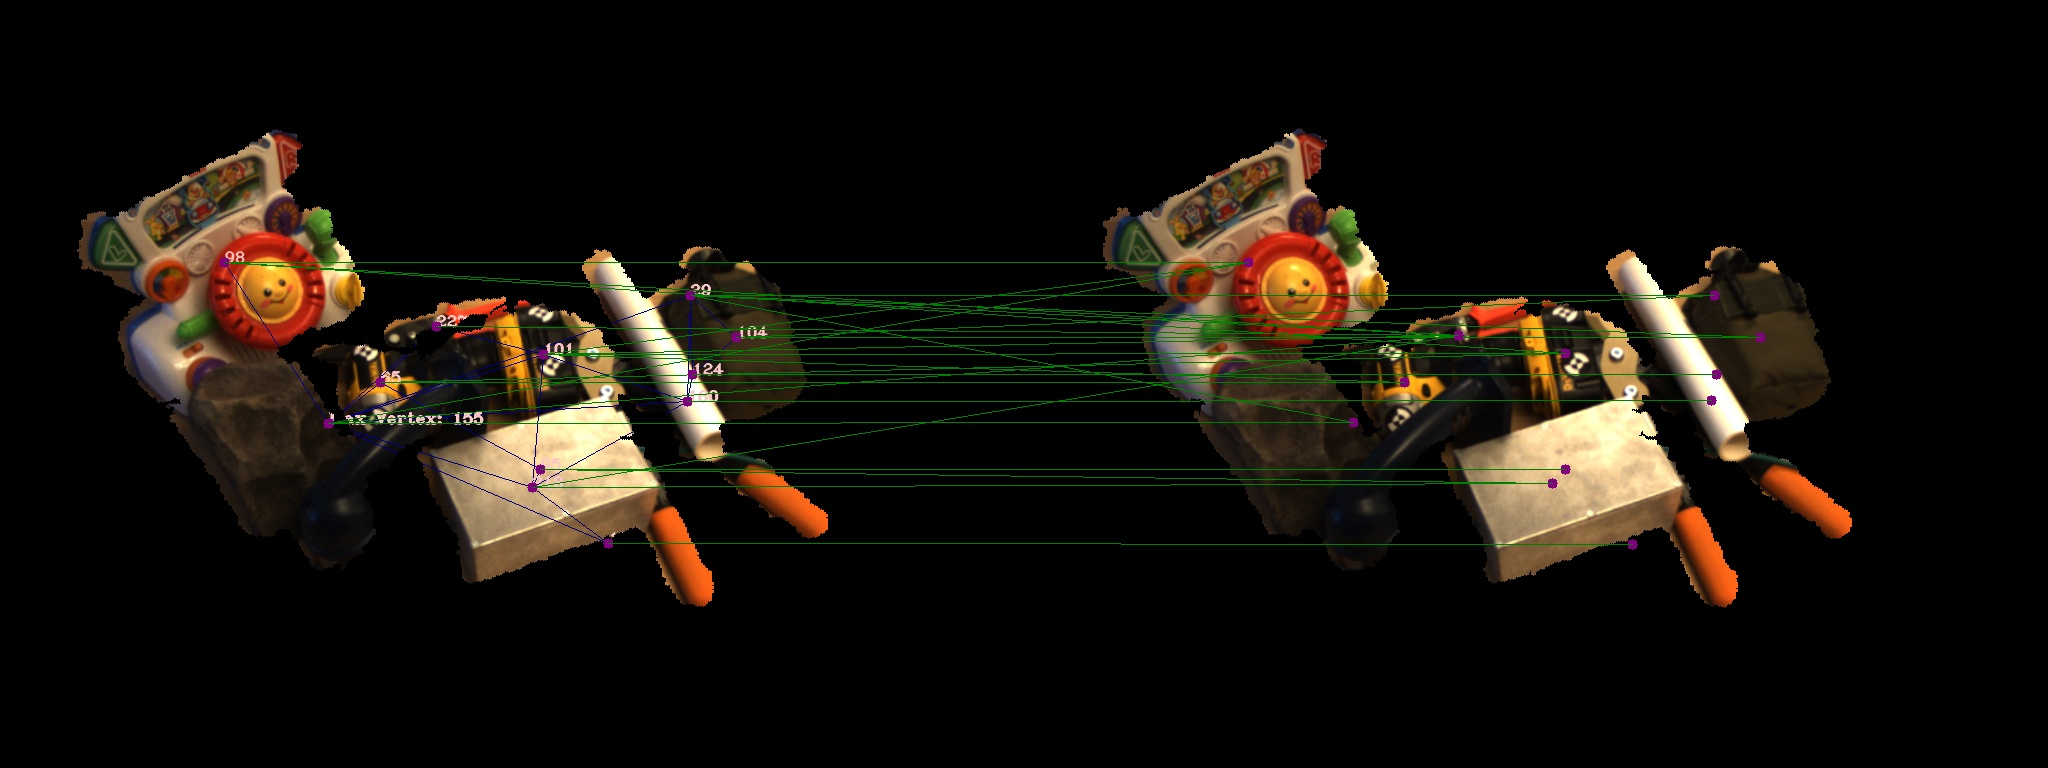
\includegraphics[width=\linewidth]{figs/correspondence.jpg}
	\caption{Show's the result of the Graph Matching algorithm after the Optical Flow update}
	\label{fig:correspondence}
\end{figure}


Once we get the updated scene graph $\mathcal{G}_{t+1}$ we perform an online policy gradient update utilizing the expected reward and the observed reward from the updated scene graph.

\subsection{Online Feature Gradient Update}
A policy gradient method is a {\bf reinforcement learning} method that directly optimizes a parametrized control policy by gradient descent. Since we use discrete actions in our approach; as opposed to performing gradient descent in policy space we peform gradient descent in feature space, thereby adapting the action selection to the current scene being observed. This is accomplished in a method similar to that employed by policy gradient approaches.

Our feature gradient also follows the gradient of the expected return where the feature weights are updated as follows.

\[
w_{k+1} = w_k + \alpha_k\bigtriangledown_w{\it J(\pi_w)}|_{w=w_k}\\
\]

where ${\it J(\pi_w)}$ the gradient on the reward is computed using regular regression

\[
\bigtriangledown_w = (\Delta W^T\Delta W)^{-1}\Delta W^T\Delta {\it J}\\
\]

The mean-subtracted reward return $\Delta {\it J}$ is obtained by subtracting the observed reward from the expected reward. The expected reward is given a function of the features weights computed using the Max Entropy learner in the offline phase. Hence the expected reward is $J(\hat{w}_k) = W^Tf(x)$. The observed reward is expected reward weighted by the variation in spectral norm of the adjacency matrix. This is given by

\[
\bar{J(w_k)} = \frac{1}{(\|A_{t+1}\| - \|A_t\|)}*\beta*J(\hat{w}_k)\\
\]

where $\beta$ is an appropriate scaling factor. The reason we use the spectral norm is because the spectral norm measures the magnitude of the largest singular value of a matrix. And to measure the similarity between two matrices we can compare their spectral norms. Hence using this logic the gradient update is performed as long as the observed adjaceny matrix and the actual adjacency matrix are different.

Once this update is performed a new action is sampled from the gibbs distribution parametrized by the updated feature weights. The actions are sampled until the variation in the spectral norm goes to zero or the feature weights top updating.
% In this section we provide a dynamic programming formulation for the single object optimization problem in (\ref{eq:sequential_optimization}). As mentioned earlier, we restrict the possible sensor poses to a discrete set $\mathcal{X}(\rho)$ of viewpoints on the viewsphere $V(\rho)$ centered at the unknown object. The state at time $t$ consists of the sensor pose $x_t \in \mathcal{X}(\rho)$ and the \textit{information state}, summarized by the sufficient statistic consisting of the probabilities for each hypothesis:
% \[
% p_i(t) = \mathbb{P}(H_i \mid Z_1=z_1,\ldots,Z_t=z_t, x_{0:t}) \in [0,1],
% \]
% where $z_{1:t}$ are the observations from the vocabulary tree. Suppose that at time $t$ the state is $(x_t,p(t))$ and the sensor decides to continue observing by moving to a new viewpoint $x_{t+1}\in\mathcal{X}(\rho)$. The new observation $z_{t+1}$ is used to update the probabilities of the hypotheses according to Bayes' rule:
% \begin{align*}
% p(t+1) &= T(p(t),x_{t+1},z_{t+1}), \text{ with $i$th component:}\\
% p_i(t+1) &= \mathbb{P}(H_i \mid z_{1:(t+1)},x_{0:(t+1)})\\
% &=\frac{\mathbb{P}(Z_{t+1} = z_{t+1} \mid x_{t+1}, H_i)\mathbb{P}(H_i \mid z_{1:t}, x_{0:t})}{\mathbb{P}(Z_{t+1} = z_{t+1}\mid x_{t+1})}\\
% &=\frac{h_i^{x_{t+1}}(z_{t+1})p_i(t)}{\sum_{j=0}^{M-1} h_j^{x_{t+1}}(z_{t+1}) p_j(t) }, \quad \forall i = 0,\ldots, M-1
% \end{align*}
% using the assumption of independence of successive observations. Supposing that $\tau$ is fixed for a moment, the terminal cost of the dynamic program can be derived after the latest observation $z_\tau$ has been incorporated in the posterior:
% \begin{align*}
% J_\tau(x_\tau,p(\tau)) &= \min_{\delta \in \{0,\ldots,M-1\}} \mathbb{E}_{Y,R} \Lambda_{\delta,j^*(Y,R)} \\
% &= \min_{\delta \in \{0,\ldots,M-1\}} \sum_{j=0}^{M-1} \Lambda_{\delta,j} p_j(\tau)
% \end{align*}
% The intermediate stage costs for $t = 0,\ldots,(\tau-1)$ are:
% \begin{align*}
% J_t(x_t,p(t)) = &\min_{v \in \mathcal{X}(\rho)} \biggl\{ c(x_t, v) + \\
% &\mathbb{E}_{Z_{t+1}} J_{t+1} (v, T(p(t), v, Z_{t+1})) \biggr\}
% \end{align*}
% Letting $\tau$ be random again and $t$ go to infinity we get the following infinite-horizon dynamic programming equation:
% \begin{align}
% \label{eq:mary_hypothesis}
% J(x,p) = &\min\biggl\{ \min_{\delta \in \{0,\ldots,M-1\}} \sum_{j=0}^{M-1} \Lambda_{\delta j} p_j, \\
% &\min_{v \in \mathcal{X}(\rho)} c(x,v) + \mathbb{E}_{Z} \{J(v,T(p,v,Z))\}\biggr\},\notag
% \end{align}
% which is well-posed by Propositions 9.8 and 9.10 in \cite{Bertsekas07_SoC}. Equation (\ref{eq:mary_hypothesis}) gives an intuition about the relationship between the cost functions $c(\cdot,\cdot)$, $\Lambda_{ij}$ and the stopping time $\tau$. If at time $t$, the expected cost of making a mistake given by $\min_{\delta \in \{0,\ldots,M-1\}} \sum_{j=0}^{M-1} \Lambda_{\delta j} p_j(t)$ is smaller than the cost of taking one more measurement, the sensor stops and chooses the minimizing hypothesis; otherwise it continues measuring.
% 
% We resort to numerical approximation techniques, which work well when the state space of the problem is sufficiently small. The decision rule $\delta(\cdot)$ can be replaced by a set of sink states $A = \{a_0,\ldots,a_{M-1}\}$ such that if the sensor goes to state $a_i$, it decides on hypothesis $H_i$ and remains there for the rest of time. Then, for $s_1, s_2 \in \mathcal{X}(\rho) \cup A$ the cost of movement and the state transition function become:
% \begin{align*}
% c'(s_1,p,s_2) &= \begin{cases}
% 				c(s_1, s_2), & s_1,s_2 \in \mathcal{X}(\rho)\\
% 				\sum_{j=0}^{M-1} p_j\Lambda_{s_2,j}, & s_1 \in \mathcal{X}(\rho), s_2 \in A\\
% 				0, & s_1=s_2 \in A\\
% 				\infty, & \text{otherwise}
% 			\end{cases}\\
% T'(p(t),s_{t+1},&z_{t+1}) = \begin{cases}
% 				T(p(t),s_{t+1},z_{t+1}), & s_{t+1} \in \mathcal{X}(\rho)\\
% 				p(t), & s_{t+1} \in A
% 			\end{cases}
% \end{align*}
% We can rewrite (\ref{eq:mary_hypothesis}) into the usual Bellman optimality equation for a POMDP:
% \[
% J(s,p) = \min_{s' \in \mathcal{X}(\rho)\cup A} \biggl\{c'(s,p,s') + \mathbb{E}_Z\{J(s', T'(p,s',Z) \} \biggr\}
% \]
% We use a point-based POMDP algorithm \cite{Kurniawati08_sarsop, Ong08_sarsop}, which approximates optimally reachable belief spaces in order to solve the problem efficiently and obtain an approximate stationary policy $\hat{\mu}: \mathcal{X}(\rho)\cup A \times [0,1]^M \rightarrow \mathcal{X}(\rho)\cup A$.

%The online procedure for using $\hat{\mu}$ is summarized in Algorithm \ref{alg:alg1}.
%\begin{algorithm}[H]
%\caption{Single Object Hypothesis Testing}
%\label{alg:alg1}
%\begin{algorithmic}[1]
%\footnotesize
%\State \textbf{Input}: Initial state $(x_0,p(0))$
%\State \textbf{Output}: Decision $\delta \in \{0,\ldots,M-1\}$
%\State
%\For{$t = 0$ to $\infty$}
%	\State $x_{t+1} \gets \hat{\mu}(x_t, p(t))$
%	\If{$x_{t+1} = a_i \in A$}
%		\State \textbf{return} $\delta \gets i$ 
%	\EndIf
%	\State Move sensor to $x_{t+1}$
%	\State $\mathcal{Q}_{t+1} \gets \phi(x_{t+1},\Omega)$
%	\State Obtain vocabulary tree score $z_{t+1}$ from $\mathcal{Q}_{t+1}$
%	\State $p(t+1) \gets T(p(t),x_{t+1},z_{t+1})$
%\EndFor
%\end{algorithmic}
%\end{algorithm}



%\section{Implementation Details}
%\section{Implementation Details}
\label{sec:impl_det}
% The previous sections developed a procedure for making a decision about the class and orientation of a single object. In this section we present the details of using this procedure to process all objects on the table as quickly as possible.
%  
% \subsection{Segmentation and data association}
% \label{subsec:seg_data_ass}
% The points $\mathcal{Q}_t$ received from the scene are clustered according to Euclidean distance by using a Kd-tree. An occupancy grid representing the 2D table surface is maintained in order to associate the clustered surfaces with new or previously seen objects. The centroid of a newly obtained surface is projected to the table and compared with the occupied cells. If the new centroid is close enough to an existing object, the surface is associated with that object and the cell is indexed by the existing object ID. Otherwise, a new object with a unique ID is instantiated.
% 
% \subsection{Coupling between objects}
% The optimization in Problem \ref{prob:active_obj_detect} is with respect to a single object but while executing it, the sensor can obtain surfaces from other objects within its field of view. We have the sensor turn towards the centroid and update the hypotheses' probabilities of every visible object. The turning is required because the observation model was trained only for a sensor facing the centroid of the object. Removing this assumption requires more training data and complicates the observation model approximation significantly. The energy used for these turns is not included in the optimization in (\ref{eq:sequential_optimization}). 
% 
% The scores obtained from the vocabulary tree are not affected significantly by scaling. This allows us to vary the radius $\rho$ of the viewsphere in order to ease the sensor movement and to update hypotheses for other objects within the field of view. The radius is set to $1$ meter by default but if the next viewpoint is not reachable, its can be adapted to accommodate obstacles and the sensor dynamics. Algorithm \ref{alg:test_pipeline} summarizes the complete hypothesis testing framework.
% 
% \begin{algorithm}[htb]
% \caption{Active Object Detection}
% \label{alg:test_pipeline}
% \begin{algorithmic}[1]
% \footnotesize
% \State \textbf{Input}: Initial sensor pose $x_0=(x_0^p,x_0^r)\in SE(3)$, object models of interest $B_2$, vector of priors $p(0) \in [0,1]^M$ for the $M$ hypotheses 
% \State \textbf{Output}: Decisions $\delta \in \{0,\ldots,M-1\}$ for every object on the table 
% \State Priority queue $pq \gets \emptyset$
% \State Current object ID $k^* \gets$ unassigned
% \For{$t = 0$ to $\infty$}
% 	\State Obtain a point cloud: $\mathcal{Q}_t \gets \phi(x_t,\Omega)$
% 	\State Cluster $\mathcal{Q}_t$ and update the table occupancy grid
% 	\For{every undecided object $k$ seen in $\mathcal{Q}_t$}
% 		\State Rotate the sensor so that $x_t^r$ faces the centroid of $k$
% 		\State Get viewsphere radius: $\rho \gets \|x_t^p - centroid(k)\|$
% 		\State Get closest viewpoint: $v^k \gets \argmin_{v \in \mathcal{X}^k(\rho)} \|x_t^p - v\|$
% 		\State Obtain a point cloud: $\mathcal{Q}^k \gets \phi(x_t,\Omega)$
% 		\State Get vocabulary tree score $z^k$ using $\mathcal{Q}^k$
% 		\State Update probabilities for object $k$: $p^k \gets T(p^k,v^k,z^k)$ 
% 		\If{$k \notin pq$}
% 			\State Insert $k$ in $pq$ according to probability $k \in B_2$, i.e. $1 - p_0^k$
% 		\EndIf
% 	\EndFor
% 	\If{$k^*$ is unassigned}
% 		\If{$pq$ is not empty}
% 			\State $k^* \gets pq.pop()$
% 		\Else
% 			\Comment{All objects seen so far have been processed.}
% 			\If{whole table explored}
% 				\State \textbf{break}
% 			\Else
% 				\State Move sensor to an unexplored area and start over
% 			\EndIf
% 		\EndIf
% 	\EndIf
% 	\State $x_{t+1} \gets \hat{\mu}(v^{k^*},p^{k^*})$
% 	\If{$x_{t+1} = a_i \in A$}
% 		\State $\delta^{k^*} \gets i$, $k^* \gets$ unassigned, Go to line $18$
% 	\EndIf
% 	\State Move sensor to $x_{t+1}$
% \EndFor
% \end{algorithmic}
% \end{algorithm}
% 

%The use of a depth sensor simplifies the segementation problem. 


%Algorithm \ref{alg:test_pipeline} summarizes the sequential optimization of the $K$ single object opimization problems. The sensor obtains an initial point cloud $\mathbb{Q}$ from the scene and clusters it. For every detected cluster, we reorient the sensor to face the cluster centroid and obtain a new point cloud. The vocabulary tree is used to obtain a score for every hypothesis from this point cloud. We repeat this process for every cluster and sort them in a priority queue according to the probability that the object is in $B_2$, i.e. ($1 - P(H_0))$. Finally, every cluster in the queue is processed using the single object hypothesis testing (See Algorithm \ref{alg:alg1}).

%TODO: - Dependent observations: Velez update, state space explosion if history of information state is kept, re-planning instead\\


%After restricting the possible sensor poses to a view-sphere and discretizing the detection scores $Z_t$, we can formulate problem (\ref{eq:mary_hypothesis}) as a POMDP by a slight modification of the state space. Let the decisions that the sensor can make be represented by actions in $A = \{a_0, \ldots, a_{M-1}\}$, each associated with one of the $M$ hypotheses. 
%The sensor pose is an observable variable by assumption and the hidden variable $(y,r)$ takes only on $M$ possible values. 




%It is assumed that the depth information from the RGB-D camera is accurate enough to provide a good estimate of an object's location. Therefore, the main task of the active detection problem is to determine if the observed point cloud $\mathcal{Q}_t$ at time $t$ is of class $\mathcal{M}$ and if so determine its orientation $r \in R$. We present a dynamic programming equation for the problem, which was specified in the problem formulation section, which casts it as an active hypothesis testing problem with a mobile sensor and fixed target. The hidden variables in our model are the true orientation $r$ and class $\mathcal{M}$ of the object.

%The active $M$-ary hypothesis testing problem problem has been addressed in literature only for a stateless sensor \cite{Javidi10_HypothesisTesting, Javidi10_MaryHypothesisTesting, Javidi11_HypothesisTesting, Javidi12_Journal}.



%\section{Experiments}
\section{Performance Evaluation}
\label{sec:experiments}
\subsection{Implementation}

% Object models, constructed using the kinect fusion algorithm from PCL, were used to construct $B_0$. The performance of the static and the active detectors were compared on synthetic scenes obtained from $B_0$. The results are summarized in Subsection \ref{subsec:static_v_active}. In Subsection \ref{subsec:real_scene}, the active framework was evaluated on several real scenes from a lab environment captured with a kinect sensor.
% 
% We used a subset of $10$ models from $B_0$ and $2$ clutter models to define $B_1$. Templates were extracted from them and were used to train the vocabulary tree. A single object of interest was used: $B_2 = \{\text{Handlebottle}\}$. The space of object yaws was discretized into $6$ bins to formulate hypotheses about the detections:
% \begin{align*}
% H_0 =& \text{ The object is \textit{not} a Handlebottle}\\
% H_i =& \text{ The object is a Handlebottle with yaw $(i-1)60$ deg}\\
% 	 &\quad\text{for } i=1,\ldots,6 
% \end{align*}
% 
% 
% \subsection{Static versus active object detection}
% \label{subsec:static_v_active}
% Fourteen synthetic scenes with $5$ objects each were constructed from the models in $B_0$. The objects were chosen so that there were $10$ instances of each hypothesis. The active detection algorithm was used with a simulated depth sensor to make decisions. Twenty five repetitions with different starting sensor poses were carried out for very object. The score from the vocabulary tree after the first observation was recorded as the decision of the static detector. The results are summarized in Fig. \ref{fig:confusion_matrix}.
% \begin{figure}[ht!]
% 	\centering
% 	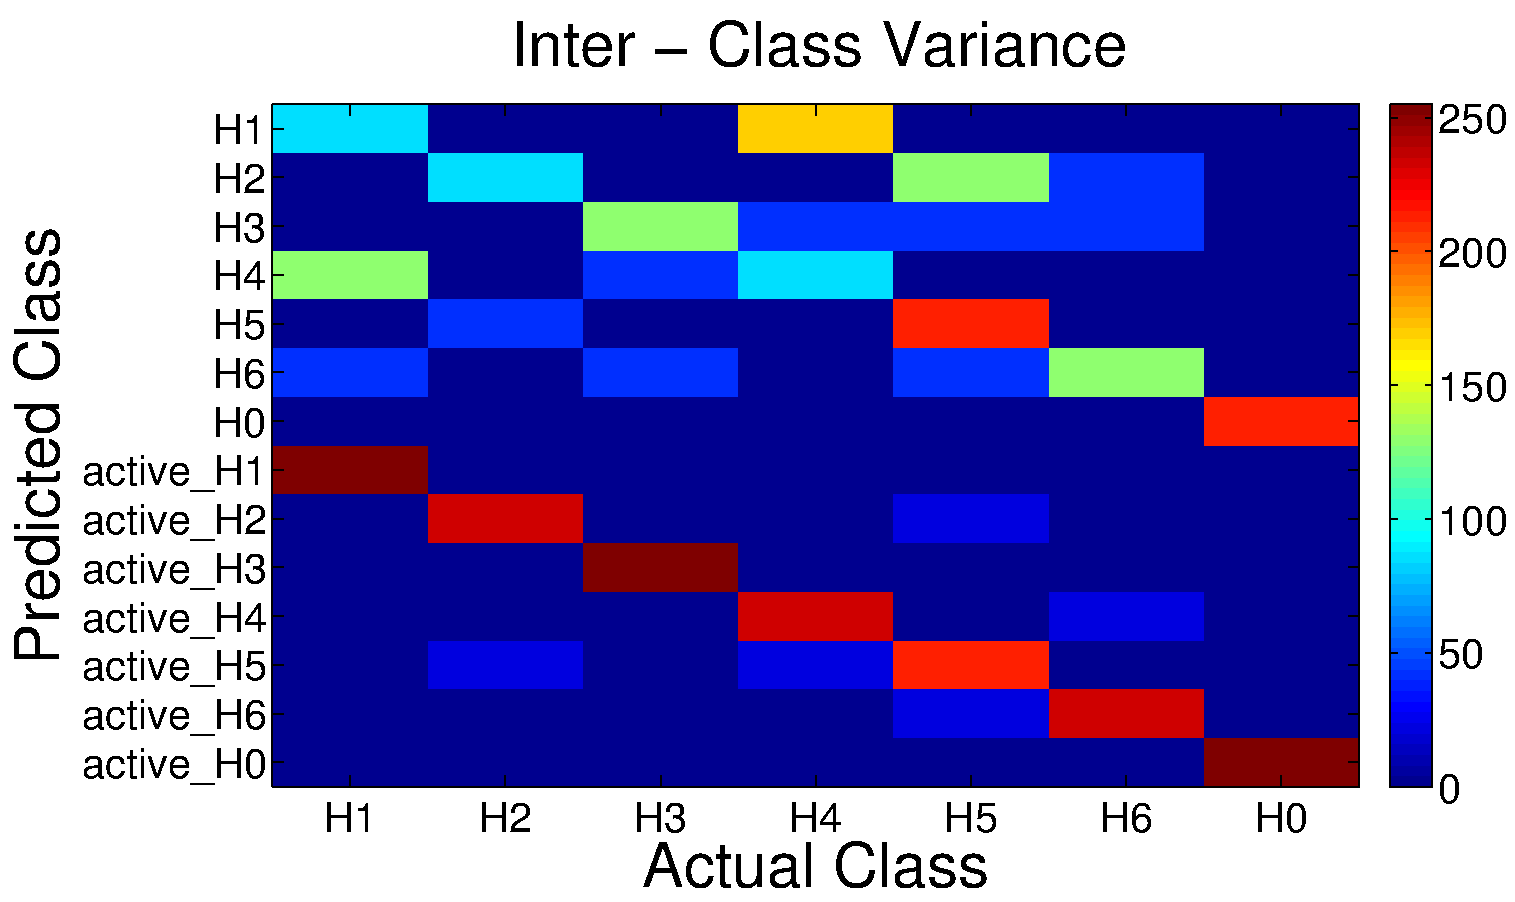
\includegraphics[width=\linewidth]{figs/active.pdf}
% 	\caption{Confusion matrix comparing the performance of the static and the active object detectors. The columns show the true hypotheses associated with each detection. The first $7$ rows present the decisions made by the static detector. The last $7$ rows show the decisions made by the active detector}
% 	\label{fig:confusion_matrix}
% \end{figure}
% The first seven rows of the confusion matrix show the decisions of the static object detector, while the results from the active framework are shown in the last seven rows. There is a marked improvement in the results when the active detection module is used.
% 
% \subsection{Experiments with real scenes}
% \label{subsec:real_scene}
% Several real scenes were captured from our lab using a kinect sensor and the fusion algorithm from PCL (See Fig. \ref{real_scene:color}). With $B_2$ and $B_1$ the same as before, the sensor's task was to detect any Handlebottles on the table and estimate their orientation. The opreration of the active detection algorithm is exemplified in Fig. \ref{real_scene:active_framework}. Since the object orientations in a real scene are not discretized a refinement step is needed if the algorithm detects an object of interest, i.e. decides on $H_i, i>0$. Then, the last observed pointcloud is aligned with the database template, which corresponds to $H_i$ using an iterative closest point algorithm. Thus, the final decision includes both a class and a continuous pose estimate.
% 
% The algorithm colors the pointcloud clusters based on its current understanding of them. Objects, which have been seen but not processed yet are colored red. The object, which is currently under evaluation is colored yellow. Once the system makes a decision about an object, it is colored green if it is of interest, i.e. in $B_2$, and blue otherwise. Fig. \ref{real_scene:result} shows a detected Handlebottle in the scene. The active framework chose hypothesis $H_3$, which corresponds to a yaw of $120\degree$. The model associated with $H_3$ is overlaid on the scene \textit{before} the orientation refinement. As you can see the two objects are already very close and the alignment procedure will produce a good \textit{continuous} orientation estimate.
% \begin{figure*}[ht!]
%   \begin{center}
%     \subfigure[Real scene captured using kinect fusion]{\label{real_scene:color}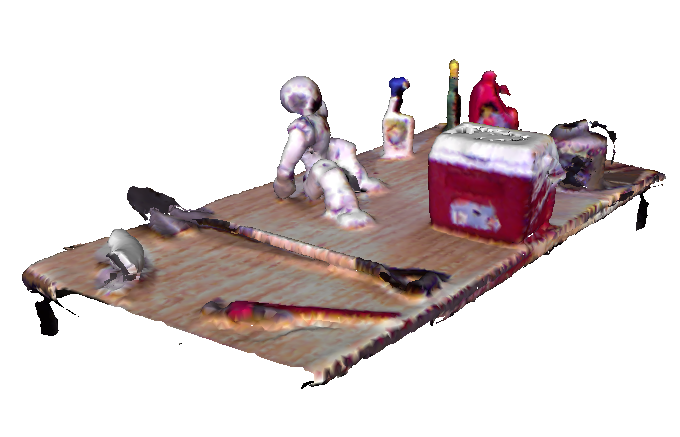
\includegraphics[width=57mm]{figs/1_real_scene.png}} 
%     \subfigure[Our algorithm's interpretation of the scene]{\label{real_scene:active_framework}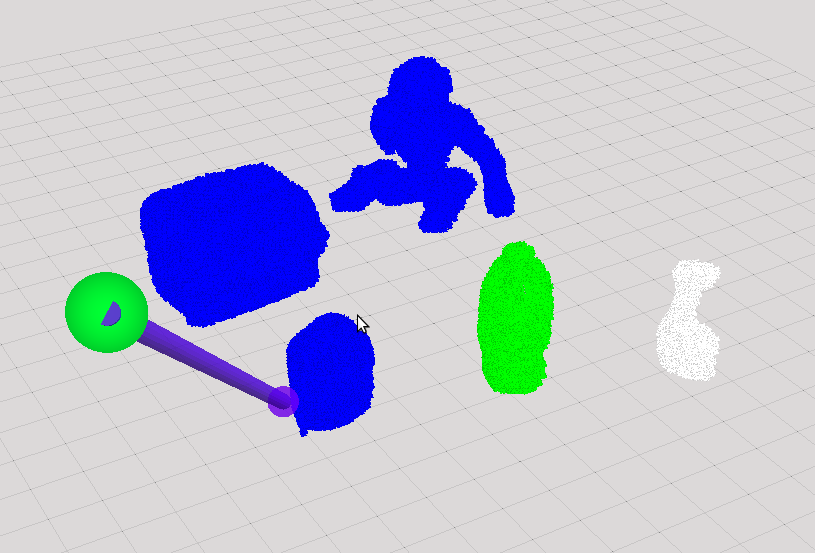
\includegraphics[width=57mm]{figs/2_decision_profile.png}}
%     \subfigure[The object of interest is detected]{\label{real_scene:result}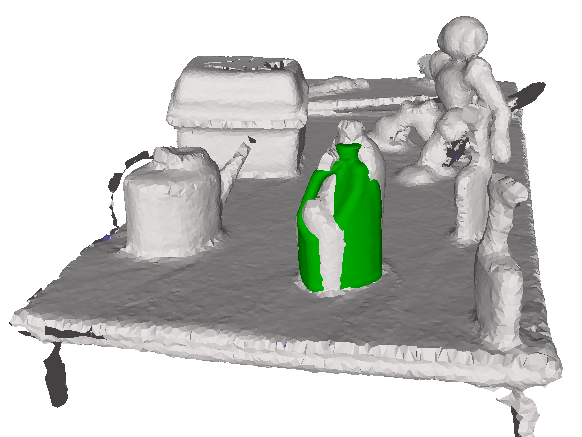
\includegraphics[width=57mm]{figs/3_final_detection.png}}
%   \end{center}
%   \caption{The active detection framework is applied to a real scene. An object is colored green if the algorithm decides it is of interest (in $B_2$) and blue otherwise. Hypothesis 3 (Handlebottle with yaw $120\degree$) was chosen for the green object in Fig. \ref{real_scene:active_framework}. The model associated with $H_3$ is overlaid on the scene in Fig. \ref{real_scene:result}  \textit{before} the final orientation refinement. See the attached video or \protect\url{http://www.seas.upenn.edu/~atanasov/ICRA2013_ActivePerception.mp4} for more details.}
%   \label{fig:real_scene}
% \end{figure*}
% 
% 
% 


%Three sets of experiments were carried out in order to evaluate the performance of our framework. Object models were constructed using a kinect sensor and were divided in testing and training classes as follows:
%\begin{align*}
%B_0 =& \{\text{Axe, Bigbox, Broom, Brush, Flowerspray, Gastank,}\\
%&\quad\text{Handlebottle, Heavyranch, Pan, Pipe, Shovel,}\\
%&\quad\text{Spadefork, Spraybottle, Watercan, Wreckbar, Robot}\}\\
%B_1 =& \{\text{Bigbox, Brush, Flowerspray, Handlebottle, Pan,}\\
%&\quad\text{Heavyranch, Pipe, Shovel, Spraybottle, Watercan}\}\\
%B_2 =& \{\text{Handlebottle}\}\\
%\end{align*}

%The object classes from $B_0$ were used to construct $14$ synthetic test scenes as described in Section \ref{sec:problem}. The performances of the static and the active object detectors were compared on all test scenes. Finally, we performed experiments using real scenes captured with the kinect sensor.















%\subsection{Evaluation of the static detector}
%\subsection{Evaluation of the active detector ion framework}
%active detection: For 14 testing scenes, run the detection thing and see the final hypotheses. Check if yaw is correct


%Our vocabulary tree is trained on templates extracted from each of these possible pose hypotheses for our object of interest. It also consists various pose templates that correspond to other objects from a limited database of objects. The tree we train has more than 1 million nodes corresponding to 11 object classes and six possible pose
%hypotheses for each class, namely from zero to 300 degrees yaw discretized at intervals of 60 degrees. In our experiements we specifically try to detect an object of class ``handlebottle'' with randomn yaw. When the vocabulary tree is queried by the active detection module, it returns a seven bit indicator
%vector corresponding to the best retreival from the vocabulary tree. For instance if the best retreival is of the ``handlebottle'' class of yaw 120 degrees then the bit corresponding to hypothesis H3 is turned on and the rest are set to zero. If the best retreival does not belong to the ``handlebottle'' class we
%set the first bit in the hypothesis indicator vector to on, i.e the bit corresponding to the zero hypothesis.
%We then use the observation model to update our posterior of the current cluster with the likelihood of this observation from the current viewpoint. In the strictly active detection case, if the final hypothesis corresponds to one of the pose hypotheses of the "handlebottle" class we use that pose hypothesis to perform a coarse to fine refinement for our final pose estimate.  

%In scenarios where the task completion hinges on the robot's ability to classify it's environment accurately based on its perceptual sensor modalities, an incorrect classification by a static object detector can adversely affect the outcome of the task. Instead in the active object
%detection scenario we let the robot move in its environment to verify its current hypothesis before performing the next task. To evaluate the comparative performance of these approaches we evaluated the output of our static object detector against the output produced by our
%active detection strategy.
%In a use case experiment we take a test scene where we are looking for a object of a specific class amongst a set of randomnly placed objects on a table. We take a scene consisting of randomly distributed objects. With our static detection pipeline we can query the vocabulary tree to get the closest template to the current surface being viewed by 
%the sensor.  These objects can consist of object classes that our vocabulary tree has been trained on and those that have never been seen before by the classifier. The pipeline is setup such that given an input scene the algorithm first extracts
%clusters above a planar surface, followed by which we update our posterior for each cluster given the data likelihood generated by the observation model. Using these posteriors we order the clusters in a priority queue and classify each cluser starting from the most likely cluster, all the way to the 
%cluster that is least likely of being the object of interest.
%We have a set of seven hypothesis of each cluster, one hypothesis corresponding to the cluster not belonging to the object class that we are trying to detect. The rest of the hypotheses correspond to the various possible coarse pose estimates of the object.






%%\begin{figure}
%%\centering
%%\subfigure{
%%	\label{sub:real_scene}
%%	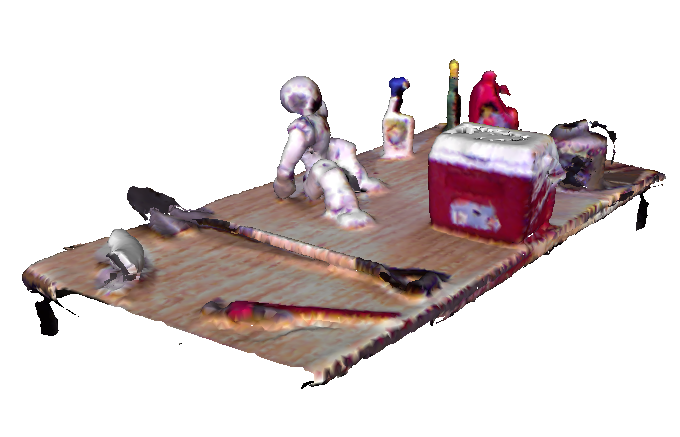
\includegraphics[width=\linewidth]{figs/real_scene_crop.png}
%%	\caption{Real scene obtained from a kinect sensor}
%%}
%%\subfigure{
%%	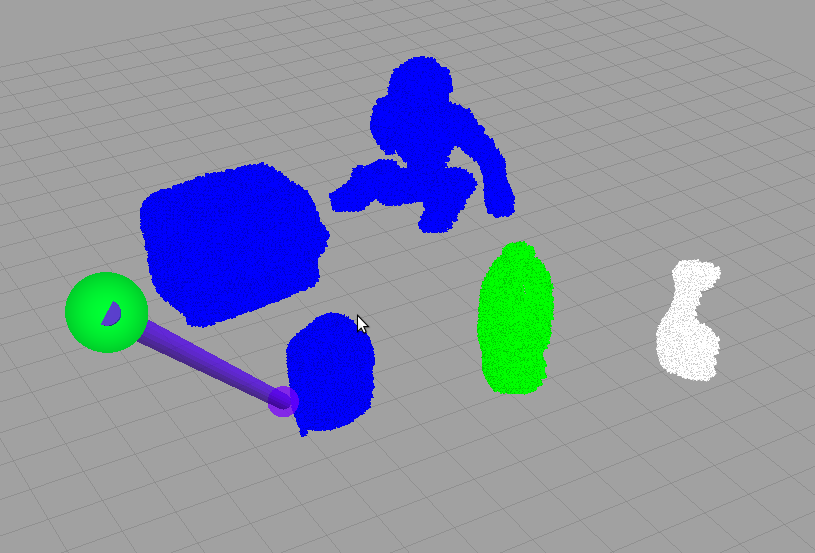
\includegraphics[width=\linewidth]{figs/decision_profile2.png}
%%	\caption{Final detections for the objects in \ref{sub:real_scene}. Blue represents non-bottle objects; green represents detected bottles. }
%%}
%%\caption{An experiment peformed using a scene captured by a kinect sensor, The top scene is the output using the kinect and the bottom images is the classification using the active detection pipeline}
%%\label{fig: scarab}
%%\end{figure}


%\subsection{Static Object Detection}
%%efficiency of our vocabulary tree by analyzing the inter-intra class variance.
%%Fig \ref{fig:templates_intra} below shows the performance of the object detection algorithm when we test for performance accuracy with respect to every template encoded.
%Our vocabulary tree is trained on templates extracted from each of these possible pose hypotheses for our object of interest. It also consists various pose templates that correspond to other objects from a limited database of objects. The tree we train has more than 1 million nodes corresponding to 11 object classes and six possible pose
%hypotheses for each class, namely from zero to 300 degrees yaw discretized at intervals of 60 degrees. In our experiements we specifically try to detect an object of class ``handlebottle'' with randomn yaw. When the vocabulary tree is queried by the active detection module, it returns a seven bit indicator
%vector corresponding to the best retreival from the vocabulary tree. For instance if the best retreival is of the ``handlebottle'' class of yaw 120 degrees then the bit corresponding to hypothesis H3 is turned on and the rest are set to zero. If the best retreival does not belong to the ``handlebottle'' class we
%set the first bit in the hypothesis indicator vector to on, i.e the bit corresponding to the zero hypothesis.
%We then use the observation model to update our posterior of the current cluster with the likelihood of this observation from the current viewpoint. In the strictly active detection case, if the final hypothesis corresponds to one of the pose hypotheses of the "handlebottle" class we use that pose hypothesis to perform a coarse to fine refinement for our final pose estimate.  

%\subsection{Hypothesis Testing for Active Object Detection}
%\label{sec:experiments}
%In our active detection strategy, as we update our posterior based on the likelihood of the observation given by the model, our active detection module either tries to take a new observation or decide on the best hypothesis. We make a decision for a cluster based on the balance betweem the cost for making a mistake and the cost of moving to an other viewpoint to get a new observation.
%In the attached video \url{:http://www.seas.upenn.edu/~atanasov/ICRA2013_ActivePerception}, if a cluster has no decision associated with it, it is colored red. When the algorithm is deciding on a cluster it is colored yellow. If it is determined to be a handlebottle the cluster color is updated
%to green if the algorithm decides on the zero hypothesis, the culster color changes to blue.

%In the figure below Fig ~\ref{fig:templates_intra}, you can see that our active detection module outperforms a static detection setup we. Tested our approach on 20 test scenes generated using a kinect and a set of random objects placed on a table.


%To study interclass variance we compare the document retreival efficiency with the best template of each class of objects and not just the best overall template as we saw in the previous experiment.
%\begin{figure}[ht!]
%	\centering
%	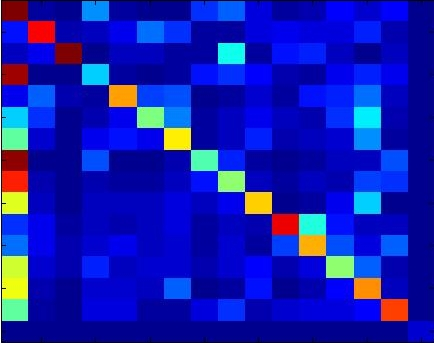
\includegraphics[height=5cm]{figs/interclass_variance.jpg}
%	\caption{Confusion Matrix for all classes in the Tree, Rows are the active and static detection outputs, Columns are the actual classes}
%	\label{fig:templates_inter}
%\end{figure} 
%As it can be noted the interclass variance is more distinct albeit there are some classes that are not accurately classified and yield false positive.




%\begin{figure}[h]
%\begin{center}$
%\begin{array}{ccc}
%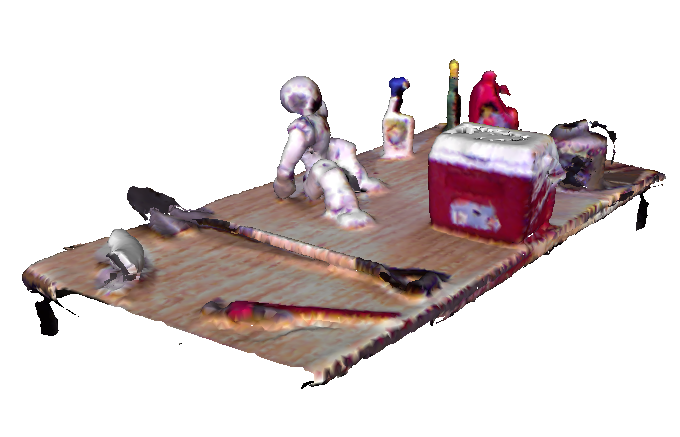
\includegraphics[width=0.3\linewidth]{figs/real_scene_crop.png} &
%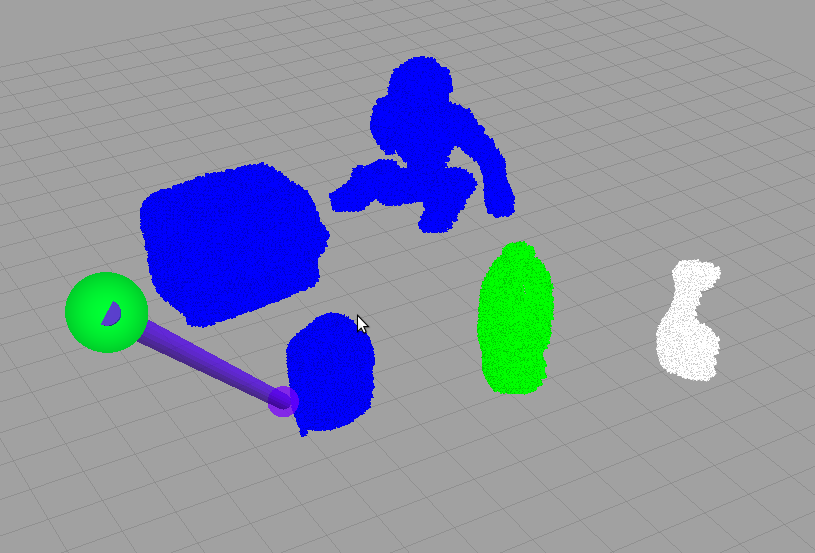
\includegraphics[width=0.3\linewidth]{figs/decision_profile2.png} &
%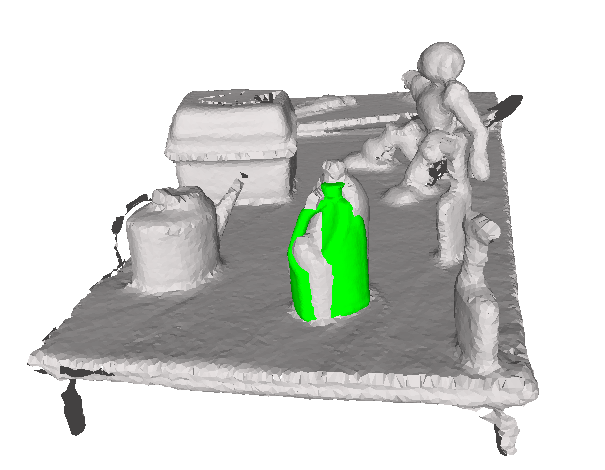
\includegraphics[width=0.3\linewidth]{figs/final_transformation.png}
%\end{array}$
%\end{center}
%\caption{my caption}
%\end{figure}






%Once a decision is made for the current cluster, the sensor moves to the next cluster in the priority queue. During the detection phase we keep a history of the estimated pose of the object returned by the coarse to fine pose refinement algorithm. We also retain a history of the visited positions in the scene to ensure that the algorithm does not oscillate between local optima.



%\begin{algorithm}[H]
%\caption{Active object detection pipeine}
%\label{pscode:pipeline}
%\begin{algorithmic}[1]
%\footnotesize
%\State \textbf{Input}: Point cloud $\mathbb{Q}$
%\State \textbf{Output}: Decision Profile $\mathbb{D}$
%\State get pointlcoud $\mathbb{Q}$ for the scene
%\State cluster $\mathbb{Q}$ into {\it k} clusters
%\State $\forall \mathbb{Q}_k \in \mathbb{Q}$ get a new sensor reading with the sensor pointed towards its centroid
%\State score the new surface $\mathbb{Q}_k$ using vocabulary tree to get $H_{0_k}$
%\State sort all $H_{0_k} \in \mathbb{Q}$ into a priority queue $\mathbb{P}$
%\State \textbf{For}: $\forall \mathbb{Q}_k \in \mathbb{P}$
%\State   Compute policy
%\State    \textbf{While}:{ best action $!=$ DECIDED}
%\State       Execute best action
%\State       Get new sensor measurement $\mathbb{Q}_k$
%\State       Update belief $H_{0_k}$
%\State   \textbf{End While}
%\State \textbf{End For}
%\end{algorithmic}
%\end{algorithm}


% \begin{algorithm}[ht]
% \caption{Active object detection pipeine}
% \label{pscode:pipeline}
% \begin{algorithmic}[1]

% \STATE {\bf Input:} Viewed Surface $s$, Object Models $\mathscr{M}_0$ and $\mathscr{M}_1$
% \STATE {\bf Output: Optimal Action: $\mathbb{A}$}
% \STATE
% \STATE $\text{Compute Model Hypothesis from Template Alignment scores for } \{s,\mathscr{M}_i\}$
% \STATE $\text{Construct octree } \mathscr{O}_i \text{ and label for each model } \mathscr{M}_i$
% \STATE Discretize viewsphere and compute set of viewpoints $\mathscr{V}$
% \FOR {$\forall v_i \in \mathscr{V}$}
% \STATE {Compute information gain $I.G(v_i)$}
% \ENDFOR 
% \STATE{\bf end for} 
% \STATE
% \STATE Compute Optimal Action $\mathbb{A}$ by solving F-HASHT
% \STATE
% \STATE{{\bf return} $\mathbb{A}$}
% \end{algorithmic}
% \end{algorithm}


%\section{Conclusion}
\section{Conclusion}
% We consider the problem of detection and pose estimation of semantically important objects versus background using a depth camera. Regardless of the quality of an object detector, the results from static recognition are affected adversely by occlusions, lighting, and scene variations. To address these issues we formulate hypotheses about the class and orientation of an unknown object and propose a soft detection strategy, in which the sensor moves to increase its confidence in the correct hypothesis. A non-myopic planning framework is used to balance the amount of energy spent for sensor motion with the benefit of decreasing the probability of incorrect decision. We demonstrated through simulation that our active detection framework outperforms static detection significantly. Additionally, we tested the algorithm on several real scenes and obtained very promising results. 
% 
% In future, work we plan to carry out additional real-world experiments in order to reproduce the analysis performed in simulation. On the theoretical side, we would like to investigate the effect of introducing sensor dynamics in the active M-ary hypothesis testing problem in order to obtain a suboptimal policy with performance guarantees.


% Bibliography
%==================================================================%
\bibliographystyle{IEEEtran}
\bibliography{bib/ICRA2014_Bibliography}
%==================================================================%

\end{document}
